\subsection{LED-Ansteuerung} \label{LED-Ansteuerung}
Die LEDs des Baseboards werden wie im Skript beschrieben mit einem PWM Timer über DMA angesteuert, um den Prozessor zu entlasten. Mit dieser Methode müssen allerdings im DMA-Buffer pro LED 24 32-Bit Integers gespeichert werden. Demnach ist eine Ansteuerung der Matrix mit 960 LEDs aufgrund des begrenzten RAM des Controlles so nicht möglich. Deshalb wurde zur Ansteuerung die SPI-Peripherie des µC verwendet. 
\begin{figure}[H]
    \centering
    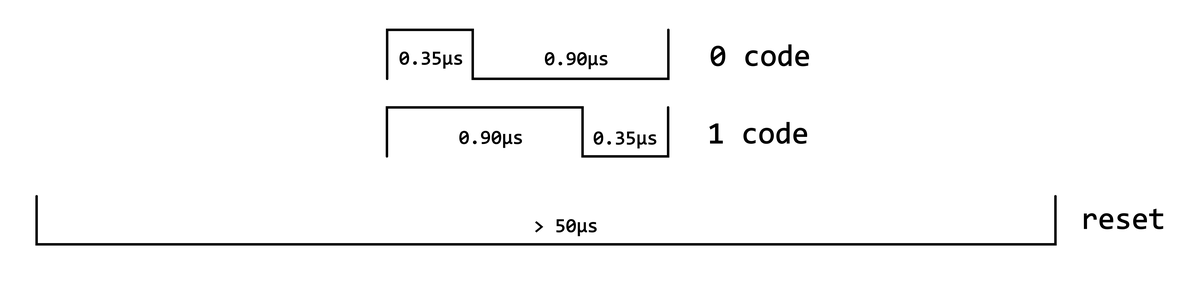
\includegraphics[page=1,width=0.85\textwidth]{images/ws2812b-timings.png} 
    \caption{Timings für die WS2812 LEDs \cite{ws2812_SPI}}
    \label{fig:ws2812b-timings}
\end{figure}
\noindent Um die timings für die LEDs zu generieren (Abb. \ref{fig:ws2812b-timings}), wurde mit 8 SPI-Bits pro Bit für das WS2812-Protokoll eine “0” als 10000000 und eine “1” als 11111100 codiert. Mit einem Prescaler für die SPI-Frequenz von 16 und einer Taktrate von 84 MHz ergibt sich eine Bitrate von 5,25 Mb/s. Da die LEDs sehr tolerant gegenüber Unterschieden im timing sind, funktionieren sie von ca. 3 bis 6 Mb/s. Durch das Nutzen des SPI-Busses mit 8 Bit pro WS2812-Bit wurde so die RAM-Auslastung auf 1/4 gegenüber der PWM-Methode verkleinert. Die Daten werden per DMA an die SPI-Peripherie übermittelt. Der Buffer wird zyklisch an die LEDs gesendet, sodass lediglich in den Buffer geschrieben werden muss und keine Aufrufen einer Funktion zur Aktualisierung der LEDs nötig ist.

\subsubsection{WS2812 DMA Library}
Die im Skript beschriebene Ansteuerung der LEDs des Baseboards wurde in einer Library realisiert. \\\\
\noindent \textbf{Konstanten:}
{\renewcommand\labelitemi{}
\begin{itemize}[leftmargin=*]
    \item \texttt{WS2812\_DMA\_*}: Verschiedene Konstanten, die die Anzahl von LEDs, Buffergrößen und die timings für die WS2812 LEDs konfigurieren.
\end{itemize}
}

\subsubsection*{Typen:}
{\renewcommand\labelitemi{}
\begin{itemize}[leftmargin=*]
    \item \texttt{PixelRGB\_t}: Eine union, die ein RGB-Pixel mit drei 8-Bit Farbkomponenten oder einen einzelnen 32-Bit Wert, für einfache Farbänderung enthält.
\end{itemize}
}
\begin{lstlisting}[style=CStyle]
typedef union
{
  struct
  {
    uint8_t b; /* blue */
    uint8_t r; /* red */
    uint8_t g; /* green */
  } c; /* color */
  uint32_t data; /* 32-bit for alignment */
} PixelRGB_t;
\end{lstlisting}

\subsubsection*{Globale Variablen}
{\renewcommand\labelitemi{}
\begin{itemize}[leftmargin=*]
    \item \texttt{WS2812\_DMA\_HANDLE}: Die \texttt{TIM\_HandleTypeDef} für des PWM timers.
    \item \texttt{ws2812\_DMA\_buffer}: DMA Buffer
    \item \texttt{ws2812\_DMA\_buffer\_ptr}: Pointer zum DMA Buffer
    \item \texttt{ws2812\_DMA\_pixels}: Ein Array vom Typ \texttt{PixelRGB\_t}, welcher die Farbwerte von jeder LED enthält.
\end{itemize}
}

\subsubsection*{Funktionen:}
{\renewcommand\labelitemi{}
\begin{itemize}[leftmargin=*]
    \item \texttt{void ws2812\_DMA\_init(void)}: Initialisiert den DMA Buffer mit dem Wert 0 (Schwarz) für jede LED.
    \item \texttt{void ws2812\_DMA\_write(PixelRGB\_t* pixel)}: Schreibt Farbdaten für einen einzelnen Pixel in den DMA Buffer.
    \item \texttt{void HAL\_TIM\_PWM\_PulseFinishedCallback(TIM\_HandleTypeDef *htim)}: Callbackfunktion, welche aufgerufen wird, wenn alle Daten aus dem DMA Buffer per PWM ausgegeben wurden. Stoppt den PWM timer.
    \item \texttt{void HAL\_TIM\_PeriodElapsedCallback(TIM\_HandleTypeDef *htim)}: Callbackfunktion für einen Timer zur Animation der LEDs.
\end{itemize}
}

\subsubsection{WS2812 SPI Library}
Die in \ref{LED-Ansteuerung} beschriebene Ansteuerung der LEDs der Matrix wurde in einer Library realisiert. \\\\
\noindent \textbf{Konstanten:}
{\renewcommand\labelitemi{}
\begin{itemize}[leftmargin=*]
    \item \texttt{WS2812\_SPI\_*}: Verschiedene Konstanten, die die Anzahl von LEDs, Buffergrößen und die timings für die WS2812 LEDs konfigurieren.
    \item \texttt{WS2812\_SPI\_FILL\_BUFFER}: Ein Macro, welches den SPI Buffer mit den Farbdaten für die WS2812 LEDs füllt.
\end{itemize}
}

\subsubsection*{Typen:}
{\renewcommand\labelitemi{}
\begin{itemize}[leftmargin=*]
    \item \texttt{PixelRGB\_t}: Eine union, die ein RGB-Pixel mit drei 8-Bit Farbkomponenten oder einen einzelnen 32-Bit Wert, für einfache Farbänderung enthält.
\end{itemize}
}

\subsubsection*{Globale Variablen}
{\renewcommand\labelitemi{}
\begin{itemize}[leftmargin=*]
    \item \texttt{WS2812\_SPI\_HANDLE}: Die \texttt{SPI\_HandleTypeDef} der SPI Peripherie.
    \item \texttt{ws2812\_SPI\_buffer}: Der Buffer für die SPI Daten.
\end{itemize}
}

\subsubsection*{Funktionen:}
{\renewcommand\labelitemi{}
\begin{itemize}[leftmargin=*]
    \item \texttt{void ws2812\_SPI\_init(void)}: Initialisiert den DMA Buffer mit dem Wert 0 (Schwarz) für jede LED und startet die SPI DMA Übertragung.
    \item \texttt{void ws2812\_SPI\_pixel(uint8\_t x, uint8\_t y, PixelRGB\_t* color)}: Setzt den Farbwert eines Pixels an den entsprechenden Koordinaten.
    \item \texttt{void ws2812\_SPI\_pixel\_all(PixelRGB\_t* color)}: Setzt alle Pixel auf den gegebenen Farbwert.
    \item \texttt{void ws2812\_SPI\_draw(PixelRGB\_t** picture, uint8\_t width, uint8\_t height)}: Setzt die LEDs auf die im zweidimensionalen Array \texttt{picture} gepseicherten Farbwerte.
    \item \texttt{void HAL\_SPI\_TxCpltCallback(SPI\_HandleTypeDef* hspi)}: Callbackfunktion, welche aufgerufen wird, wenn alle Daten aus dem DMA Buffer über SPI ausgegeben wurden. Startet die SPI DMA Übertragung erneut.
\end{itemize}
}

\subsection{Labyrinth} \label{Labyrinth}
\subsubsection{Generierung}
\subsubsection{Lösungsalgorithmus}
\subsubsection{Animation Drohne}